\section {Implementation and Technical Notes}

Python 3.6 was used to code, with modularity of components being the main focus. \\

The code has been split into modules as per the required question. For brevity, we ommit some plots, but all of these may be readily recovered by running the required question and viewing the \textit{logs} directory.

\section {Question 1}

We use \textit{scikit} to perform PCA, and \textit{pytorch } to train linear and deep auto-encoder models.

\begin{lstlisting}

\end{lstlisting}

The code to train the model is:

\begin{lstlisting}
python3 q1.py 
\end{lstlisting}

\begin{itemize}
\item Learning rate of $1e-3$, with Adam was used as the optimiser.
\item We periodically run evaluation post an epoch. 
\item Loss is MSE with respect to reconstruction.
\end{itemize}

\subsection{Accuracy and Loss Plots}

We report MSE loss convergence for the autoencoder models, along with their image reconstructions.

We observe the following:

\begin{itemize}
\item The linear autoencoder performs comparatively to PCA, however, with a different latent space representation. This is intuitive, since a PCA is the best fit linear transform, and if the network were optimal, it would mimic PCA.
\item  The deep autoencoder does much better than PCA, and has less than $1e-3$ MSE error when trained for more than 12 epochs (batch size 256). This is due to the fact that manifold learning, and not necessarily a linear transformation can occur.
\end{itemize}
\begin{figure}[!htbp]
          \begin{subfigure}
          \centering
          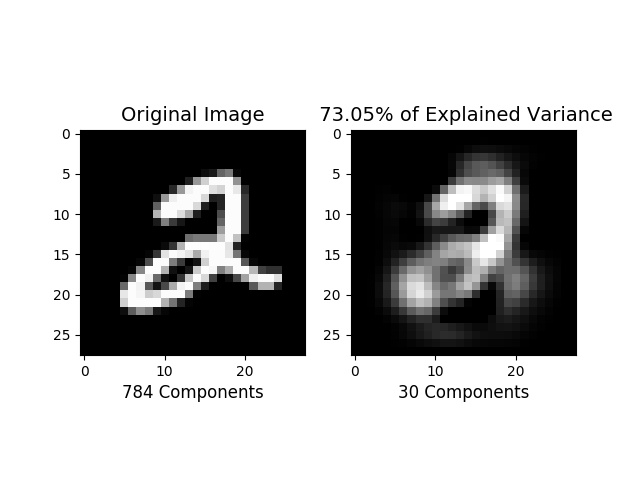
\includegraphics[angle=0,width=0.65\textwidth]{assign-4/logs/q1/pca.png}
          \caption{PCA Reconstruction, 30 components.}
          \end{subfigure}
          \end{figure}

\begin{figure}[!htbp]
          \begin{subfigure}
          \centering
          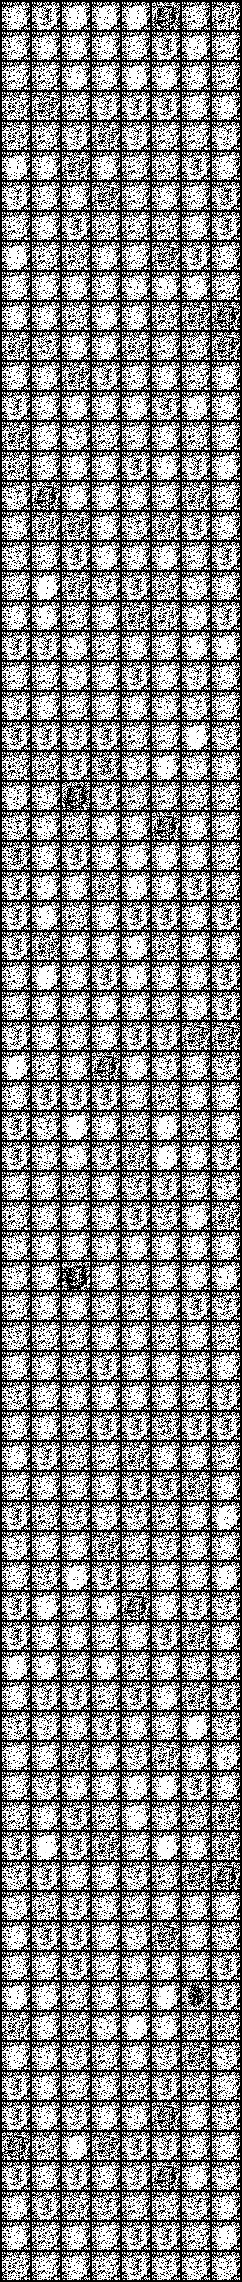
\includegraphics[angle=0,width=0.65\textwidth]{assign-4/logs/q1/linear_autoencoder/image_90.png}
          \caption{Linear Autoencoder, 1000 - 500 - 250 - 30 - 250 - 500 - 1000, reconstruction}
          \end{subfigure}
          \begin{subfigure}
          \centering
          \includegraphics[angle=0,width=0.65\textwidth]{assign-4/logs/q1/image-90.png}
          \caption{MSE Loss training convergence}
          \end{subfigure}
          \end{figure}
          
          \begin{figure}[!htbp]
          \begin{subfigure}
          \centering
          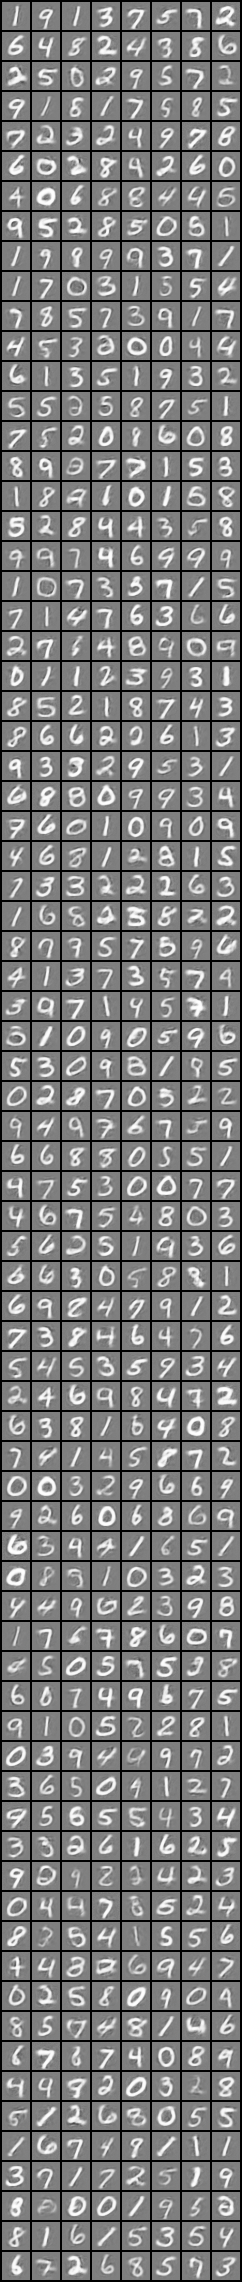
\includegraphics[angle=0,width=0.65\textwidth]{assign-4/logs/q1/deep_autoencoder/image_90.png}
          \caption{Deep Autoencoder, 1000 - 500 - 250 - 30 - 250 - 500 - 1000, reconstruction}
          \end{subfigure}
          \begin{subfigure}
          \centering
          \includegraphics[angle=0,width=0.65\textwidth]{assign-4/logs/q1/image-90.png}
          \caption{MSE Loss training convergence}
          \end{subfigure}
          \end{figure}


\section{Question 2 }

We design a standard Auto-encoder, with once hidden unit and experiment for various hidden units, of sizes: [64,128,256,512]. 
\end{itemize}

The outputs of this question may be generated by:
\begin{lstlisting}
python3 q2.py 
\end{lstlisting} 

We notice that increasing the hidden unit size increases the accuracy of reconstruction, due to better representation power. In addition, we observe poor reconstruction of non-digits. This is because the autoencoder has only learnt digit representations, and these donot generalise to non-digits.

\subsection{Loss and Accuracy Curves for H values}

\begin{figure}[!htbp]
          \begin{subfigure}
          \centering
          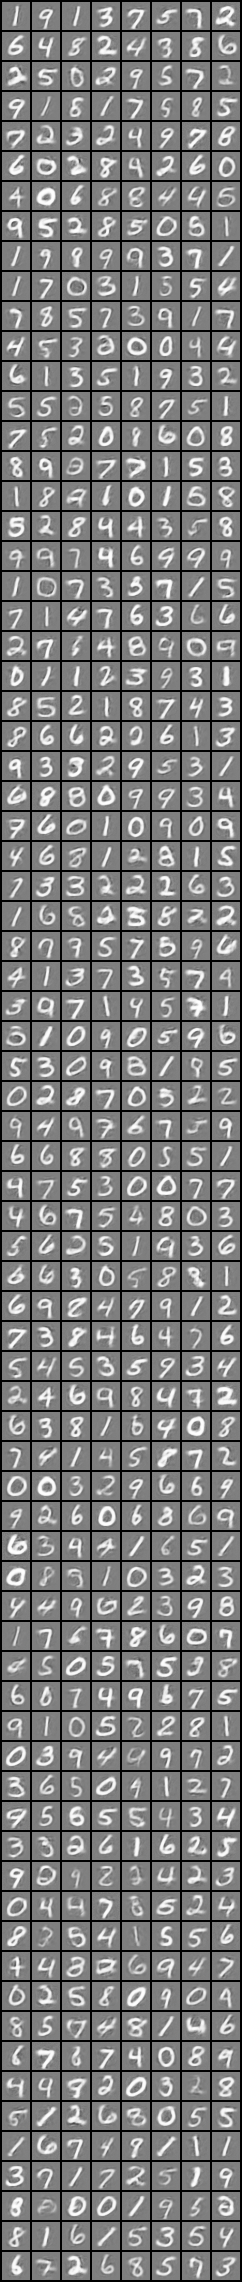
\includegraphics[angle=0,width=0.65\textwidth]{assign-4/logs/q1/deep_autoencoder/image_90.png}
          \caption{Deep Autoencoder, 1000 - 500 - 250 - 30 - 250 - 500 - 1000, reconstruction}
          \end{subfigure}
          \begin{subfigure}
          \centering
          \includegraphics[angle=0,width=0.65\textwidth]{assign-4/logs/q1/image-90.png}
          \caption{MSE Loss training convergence}
          \end{subfigure}
          \end{figure}
          \begin{figure}[!htbp]
          \begin{subfigure}
          \centering
          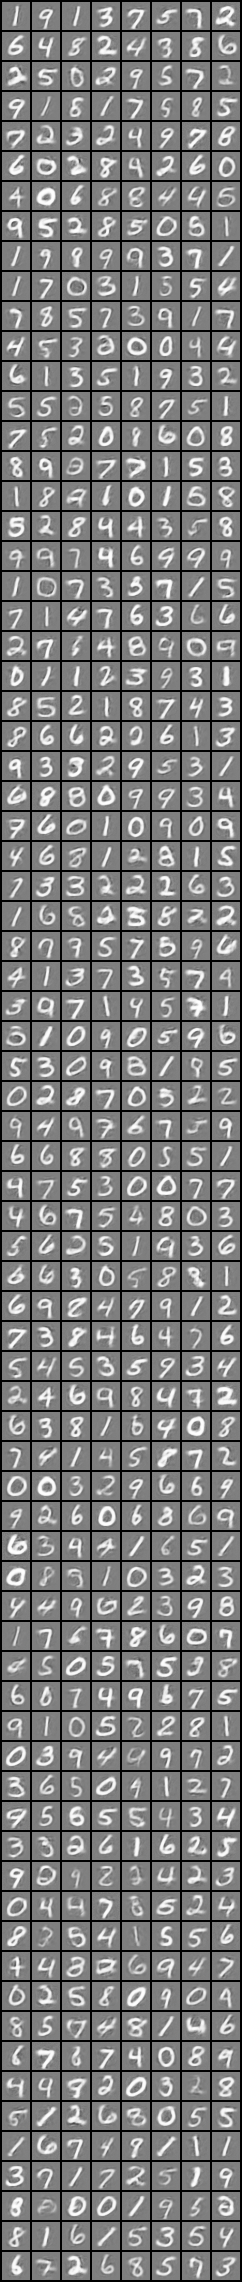
\includegraphics[angle=0,width=0.65\textwidth]{assign-4/logs/q1/deep_autoencoder/image_90.png}
          \caption{Deep Autoencoder, 1000 - 500 - 250 - 30 - 250 - 500 - 1000, reconstruction}
          \end{subfigure}
          \begin{subfigure}
          \centering
          \includegraphics[angle=0,width=0.65\textwidth]{assign-4/logs/q1/image-90.png}
          \caption{MSE Loss training convergence}
          \end{subfigure}
          \end{figure}
          
          \begin{figure}[!htbp]
          \begin{subfigure}
          \centering
          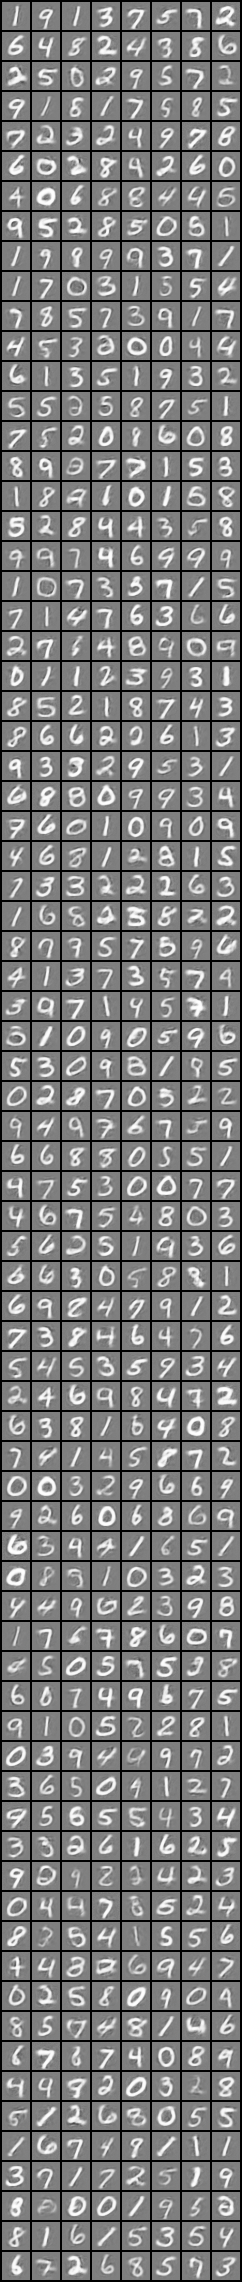
\includegraphics[angle=0,width=0.65\textwidth]{assign-4/logs/q1/deep_autoencoder/image_90.png}
          \caption{Deep Autoencoder, 1000 - 500 - 250 - 30 - 250 - 500 - 1000, reconstruction}
          \end{subfigure}
          \begin{subfigure}
          \centering
          \includegraphics[angle=0,width=0.65\textwidth]{assign-4/logs/q1/image-90.png}
          \caption{MSE Loss training convergence}
          \end{subfigure}
          \end{figure}
          
       \begin{figure}[!htbp]
          \begin{subfigure}
          \centering
          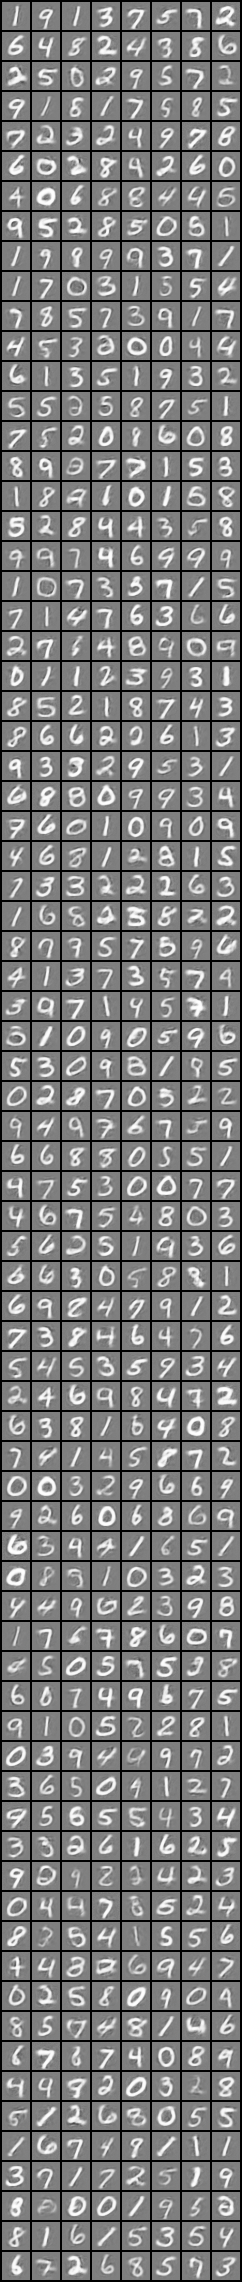
\includegraphics[angle=0,width=0.65\textwidth]{assign-4/logs/q1/deep_autoencoder/image_90.png}
          \caption{Deep Autoencoder, 1000 - 500 - 250 - 30 - 250 - 500 - 1000, reconstruction}
          \end{subfigure}
          \begin{subfigure}
          \centering
          \includegraphics[angle=0,width=0.65\textwidth]{assign-4/logs/q1/image-90.png}
          \caption{MSE Loss training convergence}
          \end{subfigure}
          \end{figure}
          

\section{Question 3}

We implement sparsity by\textit{ pytorch's }L1 weight penalisation, over the latent representation.

The outputs of this question may be generated by:

\begin{lstlisting}
python3 q3.py
\end{lstlisting} 

Hyper-parameters:
\begin{itemize}
\item  Adam optimiser, lr = 0.01, beta1 = 0.9, beta2 = 0.99
\item  Loss : MSE.
\end{itemize}

Our observations regarding non-digits persist here. We notice visible sparsity in the activations (in specific, here the latent representation).

\section{Question 4}

We implement denoising autoencoders by randomly injecting noise in the inputs, whose variance we control.

We notice better reconstructions with moderate noise, seemingly this helps make the reconstruction task less ill-posed. However, too much noise is detrimental.

The outputs of this question may be generated by:

\begin{lstlisting}
python3 q4.py
\end{lstlisting} 

The outputs are also visualised here:

\begin{figure}[!htbp]
          \begin{subfigure}
          \centering
          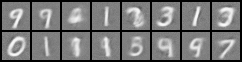
\includegraphics[angle=0,width=0.65\textwidth]{assign-4/logs/q4/deep_autoencoder_noise_0.3/image_5.png}
          \caption{Deep Autoencoder, 1000 - 500 - 250 - 30 - 250 - 500 - 1000, reconstruction}
          \end{subfigure}
          \begin{subfigure}
          \centering
          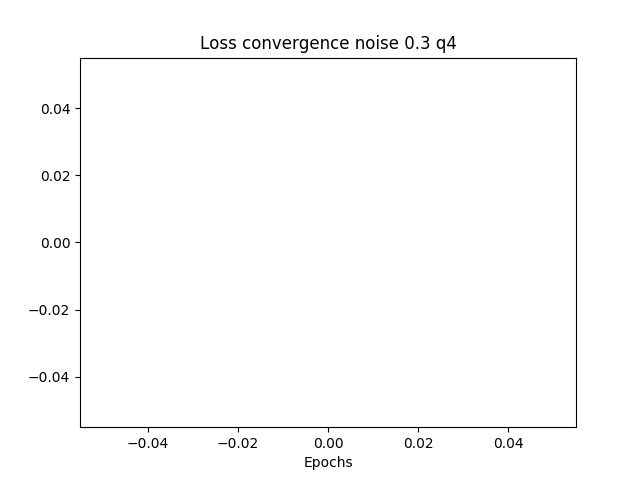
\includegraphics[angle=0,width=0.65\textwidth]{assign-4/logs/q4/convergence-noise-0.3.png}
          \caption{MSE Loss training convergence}
          \end{subfigure}
          \end{figure}
          
          \begin{figure}[!htbp]
          \begin{subfigure}
          \centering
          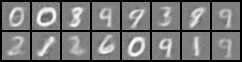
\includegraphics[angle=0,width=0.65\textwidth]{assign-4/logs/q4/deep_autoencoder_noise_0.5/image_5.png}
          \caption{Deep Autoencoder, 1000 - 500 - 250 - 30 - 250 - 500 - 1000, reconstruction}
          \end{subfigure}
          \begin{subfigure}
          \centering
          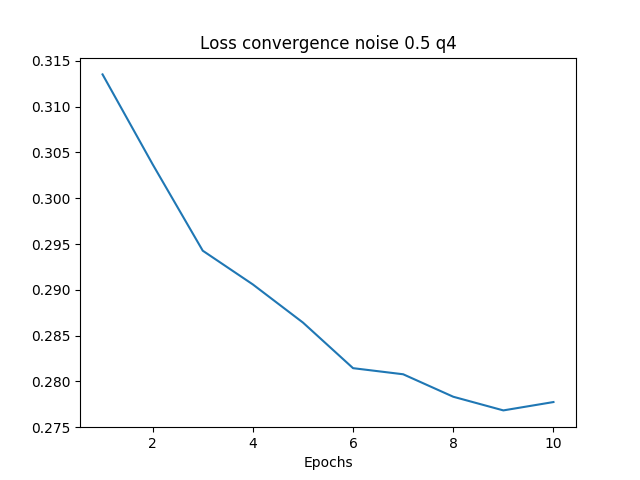
\includegraphics[angle=0,width=0.65\textwidth]{assign-4/logs/q4/convergence-noise-0.5.png}
          \caption{MSE Loss training convergence}
          \end{subfigure}
          \end{figure}
          
          \begin{figure}[!htbp]
          \begin{subfigure}
          \centering
          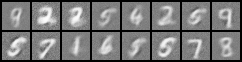
\includegraphics[angle=0,width=0.65\textwidth]{assign-4/logs/q4/deep_autoencoder_noise_0.8/image_5.png}
          \caption{Deep Autoencoder, 1000 - 500 - 250 - 30 - 250 - 500 - 1000, reconstruction}
          \end{subfigure}
          \begin{subfigure}
          \centering
          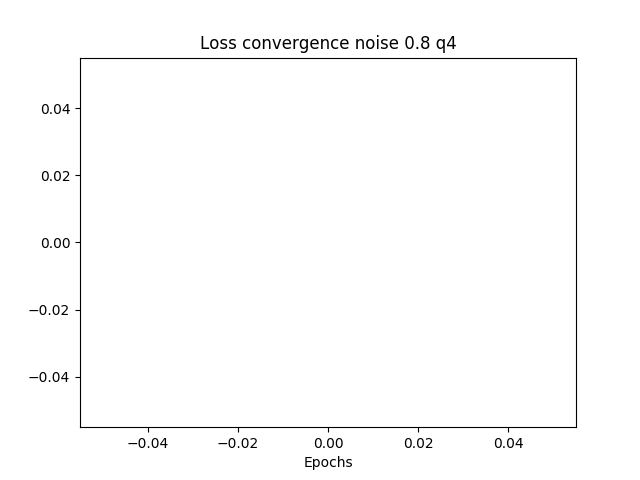
\includegraphics[angle=0,width=0.65\textwidth]{assign-4/logs/q4/convergence-noise-0.8.png}
          \caption{MSE Loss training convergence}
          \end{subfigure}
          \end{figure}
          
          \begin{figure}[!htbp]
          \begin{subfigure}
          \centering
          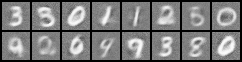
\includegraphics[angle=0,width=0.65\textwidth]{assign-4/logs/q4/deep_autoencoder_noise_0.9/image_5.png}
          \caption{Deep Autoencoder, 1000 - 500 - 250 - 30 - 250 - 500 - 1000, reconstruction}
          \end{subfigure}
          \begin{subfigure}
          \centering
          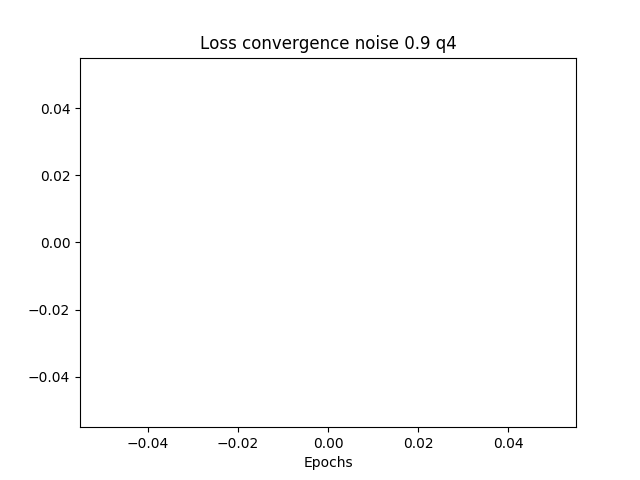
\includegraphics[angle=0,width=0.65\textwidth]{assign-4/logs/q4/convergence-noise-0.9.png}
          \caption{MSE Loss training convergence}
          \end{subfigure}
          \end{figure}
          
          
          We also visualise the hidden activations.

\section{Question 5}

\section{Question 6}

We notice that in the first case, the MSE loss visibly diverges. This is because the entire 784 coordinates donot form the image latent space, rather a subset of it. In the autoencoder case, having learnt a portion of the manifold, we donot see such a divergence.

The outputs of this question may be generated by:

\begin{lstlisting}
python3 q6.py
\end{lstlisting} 

\section{Question 7}

We use \textit{pytorch} to implement convolutional autoencoders with transposed convolution, unpooling, unpooling and transposed convolution, and reversed ordering.

We observe good reconstruction with transposed convolution and unpooling - transposed convolution. However, just unpooling and those in reversed order have poor performance.

The outputs of this question may be generated by:

\begin{lstlisting}
python3 q7.py
\end{lstlisting} 

We plot the reconstructions for unpooling reversed and unpooling - transposed convolution. (As noted above three perform similarly).

\begin{figure}[!htbp]
          \begin{subfigure}
          \centering
          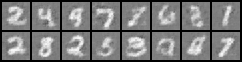
\includegraphics[angle=0,width=0.65\textwidth]{assign-4/logs/q7/deep_autoencoder_upsamp_deconv/image_5.png}
          \caption{Unpooling - Transposed Convolution Reconstruction}
          \end{subfigure}
          \begin{subfigure}
          \centering
          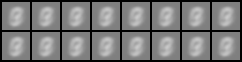
\includegraphics[angle=0,width=0.65\textwidth]{assign-4/logs/q3/deep_autoencoder_sparsity_0.1/image_5.png}
          \caption{Unpooling Reconstruction}
          \end{subfigure}
          \end{figure}
 